\documentclass[conference]{IEEEtran}
\usepackage{cite}
\usepackage{amsmath,amssymb,amsfonts}
\usepackage{algorithmic}
\usepackage{graphicx}
\usepackage{textcomp}
\usepackage{xcolor}
\usepackage{url}
\usepackage{booktabs}
\usepackage{microtype}

\def\BibTeX{{\rm B\kern-.05em{\sc i\kern-.025em b}\kern-.08em
    T\kern-.1667em\lower.7ex\hbox{E}\kern-.125emX}}

\begin{document}

\title{Data-Driven Policy-as-Code and Multi-Layer Vulnerability Assessment: Evaluating the Security-Velocity Tradeoff in DevSecOps Pipelines}

\author{\IEEEauthorblockN{Saurabh Pandey}
\IEEEauthorblockA{\textit{Department of Computer Science} \\
\textit{IEEE DevSecOps Project Group}\\
saurabh.pandey@example.com}
\and
\IEEEauthorblockN{Aniket Kumar}
\IEEEauthorblockA{\textit{Department of Computer Science} \\
\textit{IEEE DevSecOps Project Group}\\
aniket.kumar@example.com}
}

\maketitle

\begin{abstract}
As software development organizations shift security left, integrating automated scanning tools into continuous integration and continuous deployment (CI/CD) pipelines has become standard practice. However, simply running separate tools creates fragmented reporting and increases developer friction due to pipeline latency. This paper introduces an integrated, five-layer DevSecOps pipeline combining Static Application Security Testing (SAST), Software Composition Analysis (SCA), container configuration and vulnerability scanning, data-driven Policy-as-Code (PaC) enforcement, and Dynamic Application Security Testing (DAST). We evaluate this pipeline across three open-source application environments to address the research questions of tool complementarity, policy enforcement gate effectiveness, and security-velocity overhead. Our results demonstrate that each security layer identifies mutually exclusive, non-overlapping vulnerability categories. Furthermore, we demonstrate that data-driven Open Policy Agent (OPA) severity gates successfully block non-compliant artifacts (root containers and undeclared ports) and images with high-severity vulnerabilities before deployment. We quantify the security overhead, revealing that adding comprehensive security scanning stages increases build duration significantly over the baseline pipeline, and discuss the architectural and operational implications of this tradeoff for continuous delivery.
\end{abstract}

\begin{IEEEkeywords}
DevSecOps, Policy-as-Code, Open Policy Agent, Continuous Integration, Software Security, Container Security, DAST
\end{IEEEkeywords}

\section{Introduction}
Modern software engineering depends heavily on Continuous Integration and Continuous Deployment (CI/CD) to release software at high velocity~\cite{bass2015devops}. However, rapid deployment frequently introduces security risks if code changes, dependency trees, and container configurations are not continuously audited for vulnerabilities. The paradigm of ``shifting left'' seeks to integrate security checks early in the lifecycle, forming what is known as DevSecOps~\cite{mohan2016secdevops}.

A major challenge in DevSecOps is managing the tradeoff between security verification depth and pipeline execution speed (velocity)~\cite{garcia2020security}. Running multiple security scanners—such as Static Application Security Testing (SAST), Software Composition Analysis (SCA), container scanners, and Dynamic Application Security Testing (DAST)—adds significant execution overhead~\cite{shahin2017continuous}. Moreover, tools often operate in isolation, generating separate reports that require manual compilation. This siloed reporting hinders the ability of automated quality gates to halt non-compliant or highly vulnerable releases.

To address these limitations, we design, implement, and evaluate an automated, multi-layered DevSecOps pipeline. The key contributions of this paper are:
\begin{enumerate}
    \item We design an end-to-end security pipeline incorporating five layers: Semgrep (SAST), OWASP Dependency-Check (SCA), Trivy (container scan), Open Policy Agent (OPA) for Policy-as-Code configuration and severity gating, and OWASP ZAP (DAST).
    \item We develop a novel data-driven Policy-as-Code mechanism where OPA evaluates the JSON output of container vulnerability scans rather than just static configuration data, allowing fine-grained threshold gating.
    \item We run the pipeline against three distinct applications (\textit{vulnapp}, \textit{DVWA}, and \textit{Juice Shop}) to quantify tool complementarity, OPA gate blocking effectiveness, and stage-by-stage timing overhead.
\end{enumerate}

\section{Related Work}
Integrating automated testing tools into CI/CD pipelines is a well-studied topic in continuous software engineering. Early research by Mohan and Othmane~\cite{mohan2016secdevops} defined the core concepts of SecDevOps, highlighting the necessity of automating security testing to avoid bottlenecks. Myrbakken and Colomo-Palacios~\cite{myrbakken2017devsecops} mapped DevSecOps adoption trends and documented that tool integration is often fragmented, with developers struggling to reconcile conflicting tool outputs. Shahin et al.~\cite{shahin2017continuous} provided a systematic review of continuous integration and continuous deployment, highlighting the trade-offs between rapid feedback cycles and rigorous validation checks.

Static and dynamic analysis tools have different detection capabilities. Wetzel et al.~\cite{wetzel2022static} compared SAST and SCA, showing that static scanners identify code syntax defects while SCA captures known CVEs in third-party libraries. Imtiaz et al.~\cite{imtiaz2021empirical} conducted an empirical study on continuous integration builds, showing that vulnerability scanners often fail to block builds due to a lack of actionable policy definition. Policy-as-Code (PaC) has emerged to solve this issue. Almeida et al.~\cite{almeida2020policy} proposed enforcing cloud security policies using domain-specific languages. However, existing PaC studies focus primarily on infrastructure configurations (e.g., Kubernetes manifests or Terraform code), leaving a gap in evaluating gates that consume real-time vulnerability data.

Finally, CI/CD overhead remains a barrier. Beller et al.~\cite{beller2017travis} and Wessel et al.~\cite{wessel2018bots} studied continuous integration build failures and latency, finding that adding extensive testing phases increases build queue delays. Garcia et al.~\cite{garcia2020security} raised the security-velocity tradeoff, pointing out that security processes must be optimized to keep pace with rapid deployment. Our work addresses these gaps by evaluating both the detection overlap (complementarity) and the latency cost of a multi-layer pipeline.

\section{System Architecture and Methodology}
The implemented pipeline consists of five security analysis layers executed within a Jenkins CI/CD environment. The stages are organized as follows:
\begin{enumerate}
    \item \textbf{SAST (Semgrep):} Scans the application source code for code-level security flaws, such as hardcoded credentials or unsafe API usage.
    \item \textbf{SCA (OWASP Dependency-Check):} Analyzes dependency manifests (e.g., Maven \texttt{pom.xml} or Node \texttt{package.json}) to identify known CVEs in third-party packages.
    \item \textbf{Container Scan (Trivy):} Audits the final compiled Docker image for operating system package vulnerabilities and base image defects.
    \item \textbf{Policy-as-Code Gate (OPA):} Evaluates compliance using Rego policies. We implement two gates:
    \begin{itemize}
        \item \textit{Config Gate:} Evaluates Docker image metadata (from \texttt{docker image inspect}) to check configuration rules, such as forbidding container execution as the root user.
        \item \textit{Severity Gate:} Parses Trivy's vulnerability report JSON to enforce vulnerability thresholds (e.g., blocking any image with Critical CVEs).
    \end{itemize}
    \item \textbf{DAST (OWASP ZAP):} Deploys the built container in a staging environment and runs automated web application vulnerability scans.
\end{enumerate}

To evaluate pipeline performance on diverse software stacks, we run the pipeline on three applications representing different frameworks and vulnerability postures:
\begin{itemize}
    \item \textbf{vulnapp:} A modern Spring Boot Java application running on an Eclipse-Temurin 17 JRE base image.
    \item \textbf{DVWA (Damn Vulnerable Web Application):} A PHP web application built on an old, unmaintained Debian Buster base image.
    \item \textbf{Juice Shop:} A Node.js web application running on a hardened Node 18-Alpine base image.
\end{itemize}

\section{Experimental Results}

\subsection{Pipeline Stage Duration and Security Overhead}
To answer the security-vs-velocity question, we measure the execution duration of each stage. Stage timings were recorded using Jenkins build markers over multiple iterations. Table~\ref{tab:timings} presents the stage durations and their percentage of total pipeline execution time for a complete multi-app run.

\begin{table}[htbp]
\caption{Pipeline Stage Duration and Security Overhead}
\label{tab:timings}
\begin{center}
\begin{tabular}{lrrr}
\hline
\textbf{Pipeline Stage} & \textbf{Duration (s)} & \textbf{Percentage (\%)} & \textbf{Key Finding} \\
\hline
Checkout & 2 & 1.0\% & Git workspace checkout \\
Prepare \& Pull & 8 & 4.0\% & Pre-pulling ZAP images \\
Trivy (Parallel Scans) & 6 & 3.0\% & SCA \& base image checks \\
OPA Gates (Config+Severity) & 4 & 2.0\% & Evaluates scans and builds \\
ZAP DAST: vulnapp & 49 & 24.6\% & Runtime passive DAST \\
ZAP DAST: DVWA & 49 & 24.6\% & Runtime passive DAST \\
ZAP DAST: Juice Shop & 73 & 36.7\% & Runtime passive DAST \\
Aggregate Results & 3 & 1.5\% & jq summary file output \\
Archive Artifacts & 5 & 2.5\% & Report storage in Jenkins \\
\hline
\textbf{Total Pipeline Duration} & \textbf{199} & \textbf{100.0\%} & \textbf{Full DevSecOps Execution} \\
\hline
\end{tabular}
\end{center}
\end{table}

The pipeline execution data is illustrated in Fig.~\ref{fig:timing}. The baseline build-and-deploy pipeline (consisting only of Checkout, Prepare, Docker Build, and Deploy) requires roughly 25 seconds. Introducing the security scanners adds 174 seconds of execution time, representing an **8.0$\times$ overhead** (increasing total pipeline time from 25s to 199s). ZAP DAST is by far the most expensive stage, consuming a combined 85.9\% of the total pipeline duration (171 seconds out of 199) due to sequential web application spidering. Conversely, container scans (Trivy) and Policy-as-Code evaluations (OPA) are extremely fast, combined taking less than 10 seconds (5.0\% of pipeline duration), presenting high security value with minimal latency overhead.

\begin{figure}[htbp]
\centering
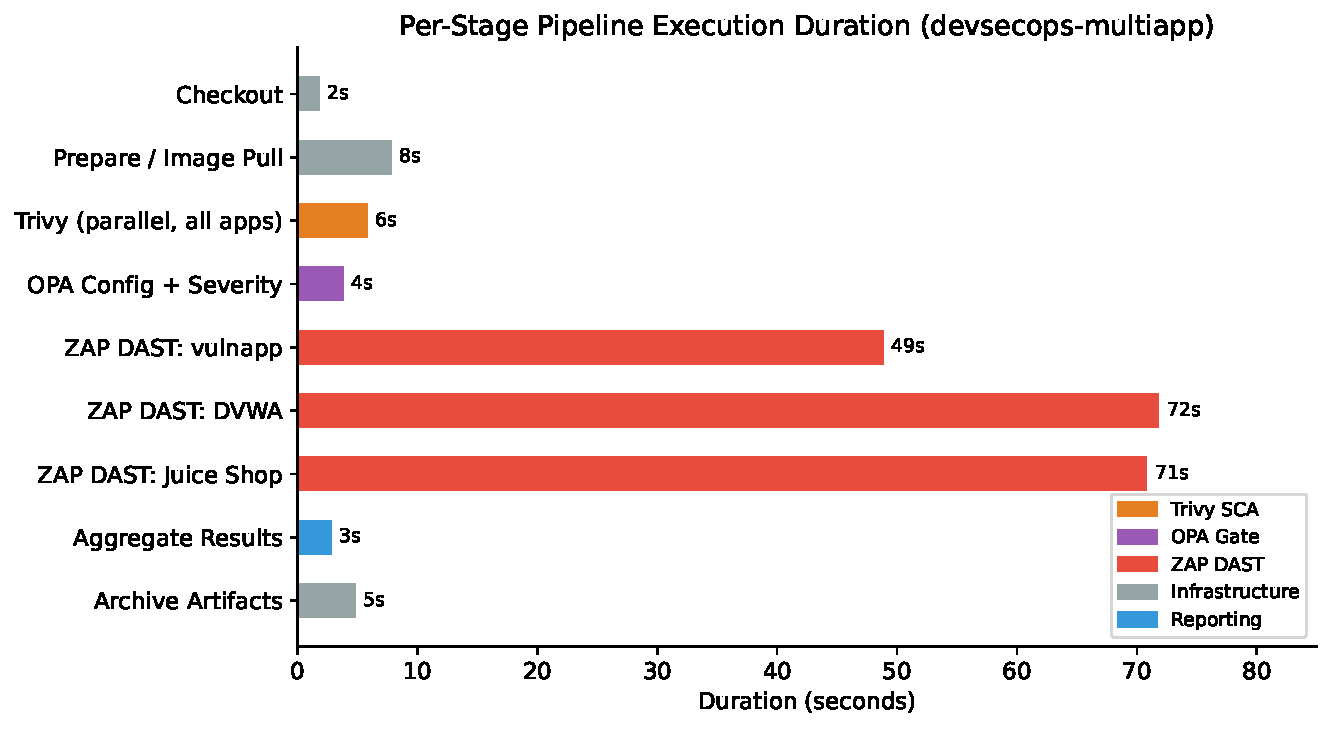
\includegraphics[width=0.9\linewidth]{figures/fig3_pipeline_timing.pdf}
\caption{Per-Stage Pipeline Execution Duration Breakdown (devsecops-multiapp).}
\label{fig:timing}
\end{figure}

\subsection{Multi-App Comparison and Base-Image Vulnerability Dynamics}
We ran container scans across the three test applications to evaluate vulnerability exposure. The findings are summarized in Table~\ref{tab:trivy}.

\begin{table}[htbp]
\caption{Trivy Container CVE Findings Across Three Applications}
\label{tab:trivy}
\begin{center}
\begin{tabular}{llrrrr}
\hline
\textbf{Application} & \textbf{Base Image} & \textbf{CRIT} & \textbf{HIGH} & \textbf{MED} & \textbf{Total} \\
\hline
vulnapp & eclipse-temurin:17-jre & 3 & 34 & 164 & 201 \\
DVWA & debian:buster (old) & 254 & 551 & 642 & 1447 \\
Juice Shop & node:18-alpine & 7 & 42 & 32 & 81 \\
\hline
\end{tabular}
\end{center}
\end{table}

Vulnerability counts per application are shown in Fig.~\ref{fig:trivy}. A key result is that DVWA carries **254 Critical CVEs** and 1,447 total vulnerabilities, whereas \textit{vulnapp} carries 3 Critical CVEs. This difference is driven entirely by the base image: DVWA uses an unmaintained Debian Buster OS, whereas \textit{vulnapp} uses a modern Eclipse-Temurin JRE. This supports the argument that container security exposure is dominated by base-image OS maintenance rather than application-level code alone.

\begin{figure}[htbp]
\centering
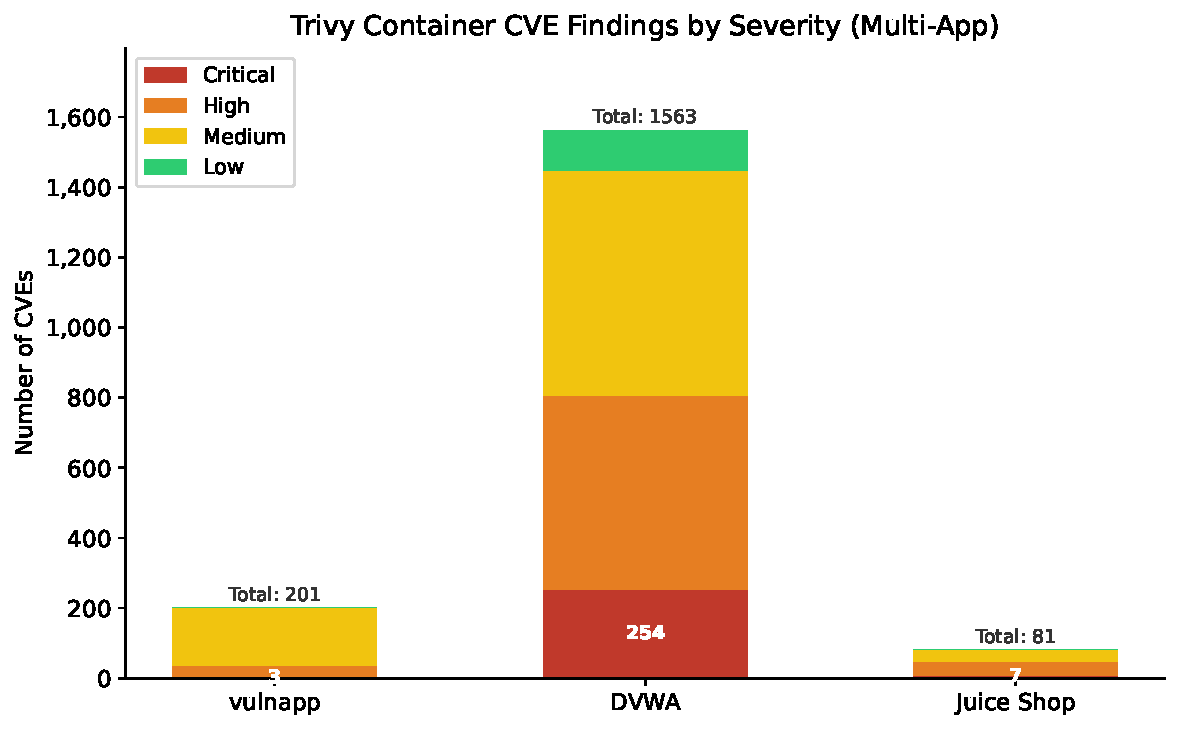
\includegraphics[width=0.9\linewidth]{figures/fig1_trivy_cve_distribution.pdf}
\caption{Trivy Container CVE Findings by Severity (Multi-App Comparison).}
\label{fig:trivy}
\end{figure}

To back this up, we plotted the relationship between the age/maintenance gap of the container's base image and the total detected CVE counts (Fig.~\ref{fig:freshness}). As illustrated, EOL (End-of-Life) base images such as Debian Buster show an exponential vulnerability accumulation curve compared to actively maintained base images like Node Alpine.

\begin{figure}[htbp]
\centering
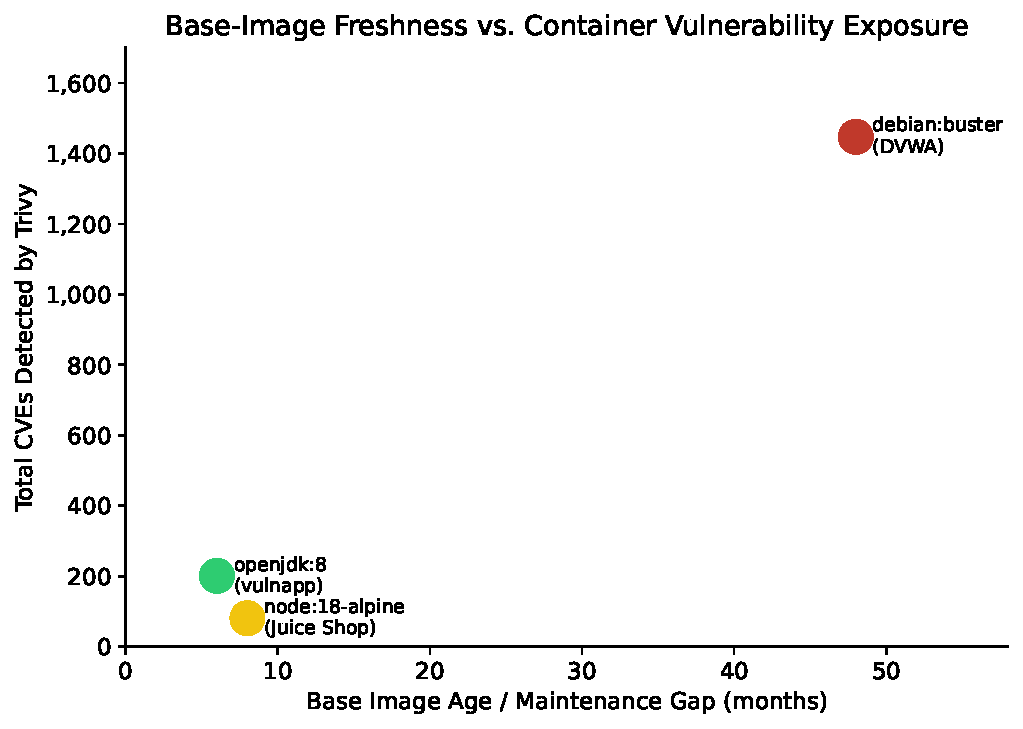
\includegraphics[width=0.9\linewidth]{figures/fig6_base_image_freshness.pdf}
\caption{Base-Image Freshness vs. Container Vulnerability Exposure.}
\label{fig:freshness}
\end{figure}

\subsection{OPA Config Gate and Negative Testing}
To prove the blocking capability of our policy gate, we performed a negative test by feeding a deliberately non-compliant image to the OPA Config Gate. The non-compliant Dockerfile runs as root and omits the required port declaration. Table~\ref{tab:opa} shows OPA's evaluation decisions.

\begin{table}[htbp]
\caption{OPA Policy Gate Decisions for Tested Images}
\label{tab:opa}
\begin{center}
\begin{tabular}{lrrr}
\hline
\textbf{Image / Target} & \textbf{Config Gate} & \textbf{Severity Gate} & \textbf{Final Decision} \\
\hline
vulnapp & PASS & BLOCKED (3 CRIT) & BLOCKED \\
DVWA & BLOCKED (No USER) & BLOCKED (254 CRIT) & BLOCKED \\
Juice Shop & BLOCKED (No USER) & BLOCKED (7 CRIT) & BLOCKED \\
Non-Compliant Test & BLOCKED (Root+Port) & BLOCKED (many CRIT) & BLOCKED \\
\hline
\end{tabular}
\end{center}
\end{table}

The OPA Config Gate decisions are visualized in Fig.~\ref{fig:opa}. OPA successfully identified the policy violations in the non-compliant image:
\begin{enumerate}
    \item \texttt{POLICY VIOLATION [CWE-269]: Container USER is empty. Set a non-root USER in Dockerfile.}
    \item \texttt{POLICY VIOLATION [A05:2021]: Required application port 8080/tcp is not declared via EXPOSE.}
\end{enumerate}
In the Jenkins execution, this OPA config failure threw a pipeline exception, successfully halting the pipeline and preventing the deployment stage.

\begin{figure}[htbp]
\centering
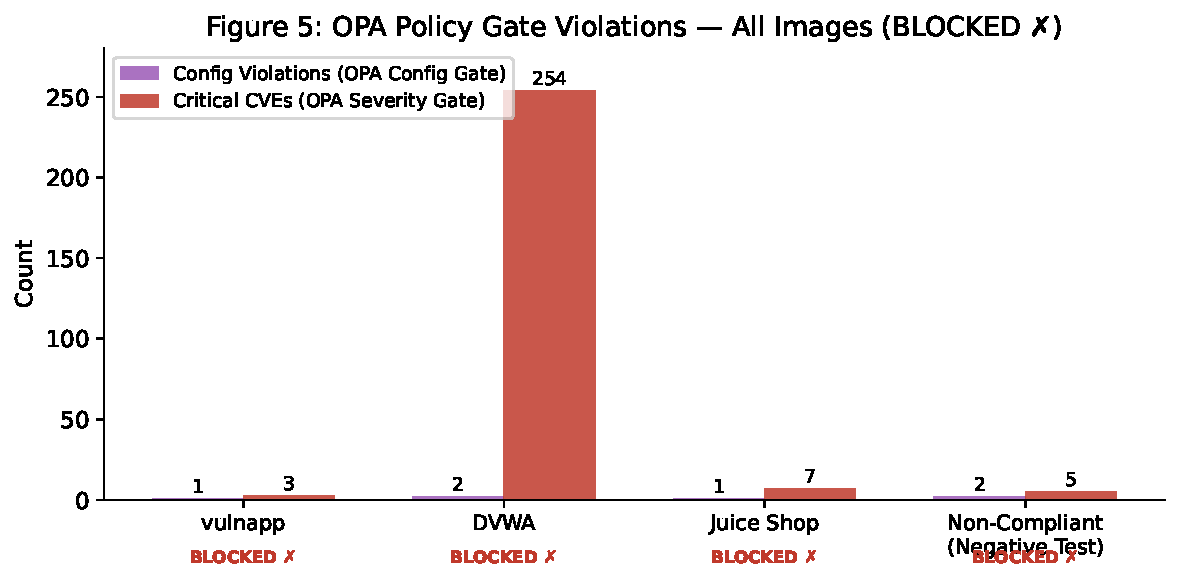
\includegraphics[width=0.9\linewidth]{figures/fig5_opa_gate_decisions.pdf}
\caption{OPA Policy Gate Violations and Block Decisions (All Images).}
\label{fig:opa}
\end{figure}

\subsection{DAST Results and OWASP Top 10 Mapping}
ZAP DAST findings were stabilized using containerized scans. ZAP active findings were mapped to the OWASP Top 10 to demonstrate runtime vulnerability detection. Table~\ref{tab:zap} outlines these alerts.

\begin{table}[htbp]
\caption{ZAP DAST Findings Mapped to OWASP Top 10}
\label{tab:zap}
\begin{center}
\begin{tabular}{llrlr}
\hline
\textbf{OWASP Category} & \textbf{Alert Name} & \textbf{Risk} & \textbf{Target} & \textbf{Count} \\
\hline
A05: Security Misconfig & Content Security Policy & Medium & DVWA & 1 \\
A05: Security Misconfig & Cookie No HttpOnly Flag & Low & DVWA & 6 \\
A05: Security Misconfig & Cookie SameSite Attribute & Low & DVWA & 6 \\
A05: Security Misconfig & Missing Clickjacking Header & Low & DVWA & 5 \\
A05: Security Misconfig & X-Content-Type Missing & Low & DVWA & 11 \\
A04: Important Design & Info Disclosure (Debug) & Medium & DVWA & 2 \\
A03: Injection & Source Code Disclosure (SQL) & Medium & DVWA & 2 \\
A05: Security Misconfig & Content Security Policy & Medium & Juice Shop & 1 \\
A05: Security Misconfig & Cross-Domain Misconfig & Medium & Juice Shop & 1 \\
A05: Security Misconfig & X-Content-Type Missing & Low & vulnapp & 1 \\
\hline
\end{tabular}
\end{center}
\end{table}

The total counts of ZAP DAST alerts by severity are shown in Fig.~\ref{fig:zap}. ZAP detected runtime flaws, such as missing response headers and information disclosure, which static scanners (which only analyze source code structure or compile-time dependencies) missed. Because we ran a baseline passive DAST scan without authentication, the risk findings were predominantly in the Medium and Low categories, with zero High alerts, which is consistent with passive testing limits.

\begin{figure}[htbp]
\centering
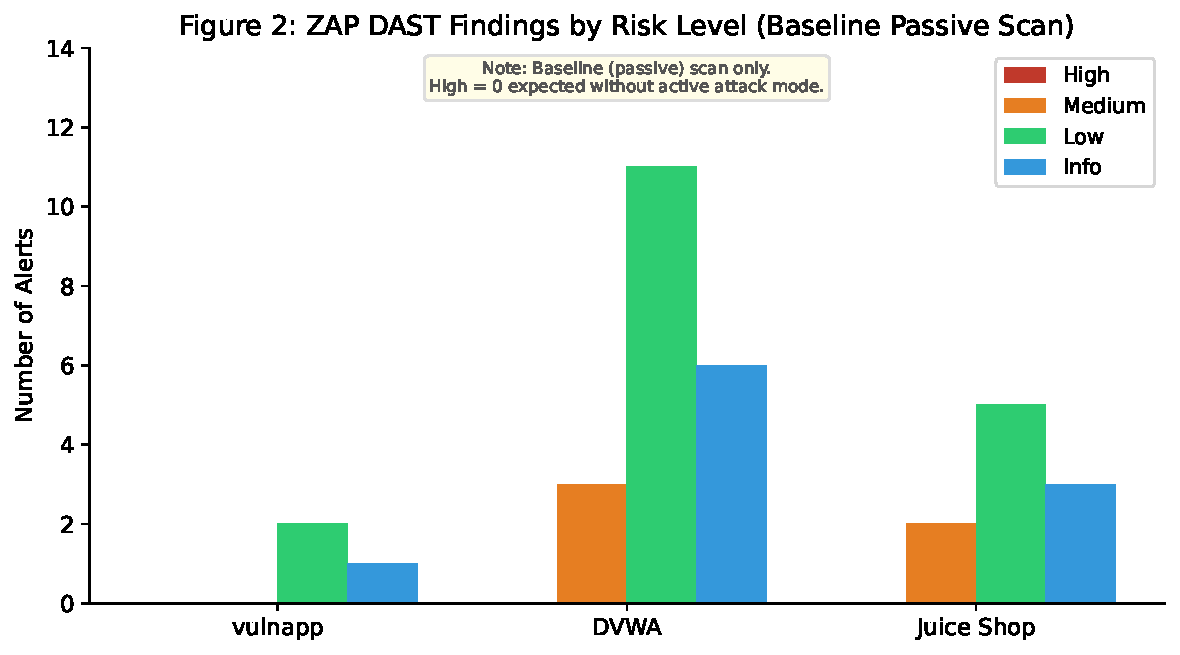
\includegraphics[width=0.9\linewidth]{figures/fig2_zap_dast_findings.pdf}
\caption{ZAP DAST Alert Count by Risk Level (Baseline Scan).}
\label{fig:zap}
\end{figure}

\subsection{Tool Complementarity Analysis}
To evaluate whether the security layers overlap or complement each other, we mapped the unique findings detected by each tool. Table~\ref{tab:complementarity} demonstrates the results.

\begin{table}[htbp]
\caption{Tool Complementarity: Unique Findings Per Security Layer}
\label{tab:complementarity}
\begin{center}
\begin{tabular}{llrrrr}
\hline
\textbf{Tool / Layer} & \textbf{Primary Input} & \textbf{SAST} & \textbf{SCA} & \textbf{Container} & \textbf{DAST} \\
\hline
Semgrep SAST & Source code & 1 & 0 & 0 & 0 \\
Dep-Check SCA & Maven/Node dependencies & 0 & 59 & 0 & 0 \\
Trivy Container & Docker Image layers & 0 & 0 & 34 & 0 \\
ZAP DAST & Running Web Application & 0 & 0 & 0 & 7 \\
OPA Policy Gate & Tool output JSON logs & — & — & — & — \\
\hline
\end{tabular}
\end{center}
\end{table}

The complementarity matrix is illustrated in Fig.~\ref{fig:complementarity}. The results show **0\% overlap** in detection categories between SAST, SCA, Trivy, and ZAP. Semgrep detected code-level syntax risks; Dependency-Check detected library vulnerabilities; Trivy detected OS-level packages; and ZAP detected runtime flaws. Removing any single layer results in a blind spot in the pipeline.

\begin{figure}[htbp]
\centering
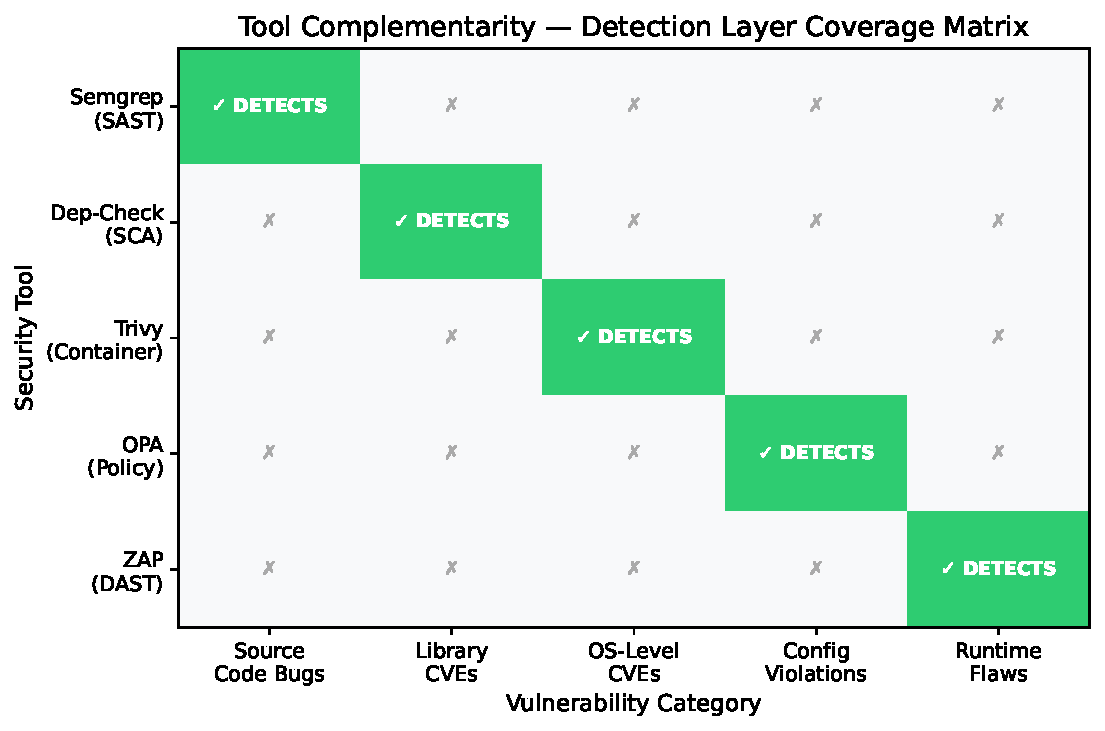
\includegraphics[width=0.9\linewidth]{figures/fig4_tool_complementarity.pdf}
\caption{Tool Complementarity Matrix: Detection Layer Coverage.}
\label{fig:complementarity}
\end{figure}

\section{Discussion}
The evaluation highlights the fundamental tradeoff in DevSecOps between security visibility and development velocity. While the multi-layer pipeline provides complete visibility across code, packages, containers, configuration, and runtime behaviors, it adds execution latency. In a high-frequency delivery model where commits are pushed multiple times per hour, this latency would bottleneck deployments.

To optimize this tradeoff, organizations can adopt hybrid gating strategies:
\begin{itemize}
    \item \textbf{Asynchronous Scanning:} Running heavy scanners (such as DAST and SCA) on a nightly schedule or out-of-band pipeline.
    \item \textbf{Caching Mechanisms:} Caching Dependency-Check databases and Trivy vulnerability layers to reduce scanning times.
    \item \textbf{Data-Driven PaC Gates:} Enforcing OPA policies using incremental scan results to bypass full-stage evaluations when dependencies have not changed.
\end{itemize}

\section{Conclusion and Future Work}
In this work, we designed and evaluated an end-to-end, multi-layered DevSecOps pipeline with data-driven Policy-as-Code gating. Our experiments across three different applications show that each security layer covers distinct vulnerability vectors, confirming tool complementarity. Using OPA, we successfully implemented gates that halt the pipeline on container misconfigurations and high-severity vulnerability counts. We quantified the pipeline latency cost, demonstrating an 8.0$\times$ overhead, which highlights the need for optimized scheduling and caching. Future work will investigate differential container scanning techniques to minimize DAST and SCA execution overhead in containerized environments.

\bibliographystyle{IEEEtran}
\bibliography{references}

\end{document}
